% TEMPLATE for Usenix papers, specifically to meet requirements of
%  USENIX '05
% originally a template for producing IEEE-format articles using LaTeX.
%   written by Matthew Ward, CS Department, Worcester Polytechnic Institute.
% adapted by David Beazley for his excellent SWIG paper in Proceedings,
%   Tcl 96
% turned into a smartass generic template by De Clarke, with thanks to
%   both the above pioneers
% use at your own risk.  Complaints to /dev/null.
% make it two column with no page numbering, default is 10 point

% Munged by Fred Douglis <douglis@research.att.com> 10/97 to separate
% the .sty file from the LaTeX source template, so that people can
% more easily include the .sty file into an existing document.  Also
% changed to more closely follow the style guidelines as represented
% by the Word sample file.

% Note that since 2010, USENIX does not require endnotes. If you want
% foot of page notes, don't include the endnotes package in the
% usepackage command, below.

% This version uses the latex2e styles, not the very ancient 2.09 stuff.

%%%%%%%%%%%%%%%%%%%%%%%%%%%%%%%%%%%%%%%%%%%%%%%%%%%%%%%%%%%%%%%%%%%%%%
%  Packages
%%%%%%%%%%%%%%%%%%%%%%%%%%%%%%%%%%%%%%%%%%%%%%%%%%%%%%%%%%%%%%%%%%%%%%


\documentclass[letterpaper,twocolumn,10pt]{article}
\usepackage{usenix,epsfig,endnotes}
\usepackage{url}
\usepackage{multirow}
\usepackage{booktabs}
\usepackage{color}
\usepackage[normalem]{ulem}
\usepackage[usenames,dvipsnames]{xcolor}
\usepackage{pifont}
\usepackage{graphicx}
\usepackage{makecell}
\usepackage{xspace}

\usepackage[small,compact]{titlesec}
\usepackage{flushend}

\usepackage[shortlabels]{enumitem}
\setlist[itemize]{leftmargin=0.15in}

\titlespacing{\section}{0pt}{3pt}{3pt}
\titlespacing{\subsection}{0pt}{2pt}{2pt}
\titlespacing{\subsubsection}{0pt}{1pt}{1pt}

\newcommand{\urlwofont}[1]{\underline{\urlstyle{same}\url{#1}}}
\newif\ifrev
%  COMMENT OUT NEXT LINE TO HIDE TODOs AND COMMENTS
\revtrue

\newcommand{\lip}{\emph{Lock-in-Pop}\xspace}
\newcommand{\redact}{[redacted]}
\ifrev
  \newcommand{\brendan}[1]{{\color{purple} [Brendan: #1]}}
  \newcommand{\cappos}[1]{{\color{red} [Justin: #1]}}
  \newcommand{\lois}[1]{{\color{magenta} [Lois: #1]}}
  \newcommand{\yiwen}[1]{{\color{OliveGreen} [Yiwen: #1]}}
  \newcommand{\todo}[1]{{\color{Orange} [TODO: #1]}}
\else
  \newcommand{\brendan}[1]{}
  \newcommand{\yanyan}[1]{}
  \newcommand{\cappos}[1]{}
  \newcommand{\lois}[1]{}
  \newcommand{\yiwen}[1]{}
  \newcommand{\todo}[1]{}
\fi

\setlist[itemize]{leftmargin=*}

%\setlength{\textfloatsep}{6mm}
\setlength{\abovecaptionskip}{1mm}

\begin{document}


%don't want date printed
%\date{}


%%%%%%%%%%%%%%%%%%%%%%%%%%%%%%%%%%%%%%%%%%%%%%%%%%%%%%%%%%%%%%%%%%%%%%
%  Title and Authors
%%%%%%%%%%%%%%%%%%%%%%%%%%%%%%%%%%%%%%%%%%%%%%%%%%%%%%%%%%%%%%%%%%%%%%


%make title bold and 14 pt font (Latex default is non-bold, 16 pt)
\title{\Large \bf{Lock-in-Pop: Securing Privileged Operating System Kernels by Keeping on the Beaten Path}}


%for single author (just remove % characters)
%\author{
%{\rm Yiwen Li}
%New York University \\
%liyiwen@nyu.edu
%\and
%{\rm Brendan Dolan-Gavitt}
%New York University\\
%brendandg@nyu.edu
%\and
%{\rm Sam Weber}
%New York University\\
%samweber@nyu.edu
%\and
%{\rm Justin Cappos}
%New York University
%jcappos@nyu.edu
%} % end author

\author{{\rm Yiwen Li} \qquad {\rm Brendan Dolan-Gavitt} \qquad 
{\rm Sam Weber} \qquad {\rm Justin Cappos} 
\\ New York University}


\maketitle


% Use the following at camera-ready time to suppress page numbers.
% Comment it out when you first submit the paper for review.
\thispagestyle{empty}

\pagenumbering{gobble}

%%%%%%%%%%%%%%%%%%%%%%%%%%%%%%%%%%%%%%%%%%%%%%%%%%%%%%%%%%%%%%%%%%%%%%
%  Sections
%%%%%%%%%%%%%%%%%%%%%%%%%%%%%%%%%%%%%%%%%%%%%%%%%%%%%%%%%%%%%%%%%%%%%%


\subsection*{Abstract}

%Virtual machines (VMs) are widely used in practice, in part for their ability to
%isolate potentially untrusted code from the rest of a system.
%Recently, library OSes and containers have also presented promising security options.
%
%However, it is often possible to trigger zero-day flaws
%in the host Operating System (OS) from inside of such virtualized systems.
%

%In this paper, we offer a new insight about where security bugs lie. By observing that the OS kernel paths accessed
%by popular applications in everyday use contain significantly fewer security bugs than less-used paths, 
%we devise a design that allows applications to run more securely in VMs on top of a vulnerable host OS.
%Furthermore, We
%leverage this observation to devise the \lip design, which
%\textbf{\textit{locks}} an application, and the POSIX implementation that services it, into
%accessing only the well-used \textbf{\textit{popular}} portion of the kernel.  Using the \lip model, we
%implement a prototype virtual machine called Lind.
%
%We compare Lind and three other virtualized systems that were
%available at the release of Linux kernel version 3.14.1, and evaluate
%their effectiveness in containing the zero-day kernel bugs that have been discovered
%since then.
%
%Our results show that Lind can prevent the triggering of zero-day kernel bugs significantly better
%than an existing library OS (Graphene) and containers such as Docker and LXC.

Virtual machines (VMs) that try to isolate untrusted code are widely used in practice. 
However, it is often possible to trigger zero-day flaws
in the host Operating System (OS) from inside of such virtualized systems.
%
In this paper, we propose a new security metric showing strong correlation between ``popular paths'' 
and kernel vulnerabilities. We verified that the OS kernel paths accessed 
by popular applications in everyday use contain significantly fewer security bugs than less-used paths.  We then demonstrate that this observation is
practically useful by building a prototype system which \textbf{\textit{locks}} an
application into only using \textbf{\textit{popular}} OS kernel paths.  By doing so, we
demonstrate that
we can prevent the triggering of zero-day kernel bugs
significantly better than three other competing approaches, and argue that
this is a practical approach to  secure system design.

\section{Introduction}
\label{sec.introduction}

The number of attacks involving the exploitation of zero-day vulnerabilities more than doubled 
from 2014 to 2015 \cite{zero-day}. Skilled hackers can find a security flaw in a system and use it to hold the system's users hostage, e.g., 
by gaining root access and compromising the host \cite{linux-0day}. Similarly, zero-day
vulnerabilities can be exploited \cite{fbi-0day} or their presence not be acknowledged \cite{nsa-0day} 
by government agencies, thus rendering millions of devices vulnerable.

In theory, running a program in an operating system-level virtual machine (OSVM) like Docker \cite{Docker} or LXC \cite{LXC} should
prevent bugs in the host OS kernel from triggering. 
However, the isolation provided by such systems is not the whole answer and faces some significant drawbacks. 
To be effective, OSVM's software must not contain any bugs that could allow the program to escape the machine's containment 
and interact directly with the host OS. 
Unfortunately, these issues are very common in OSVMs, with 14 CVE vulnerabilities confirmed for Docker \cite{Docker-Vulnerabilities} since 2014. 
The large amount of complex code needed to run such a system increases the odds that flaws will be present, and, in turn, 
that tens of millions of user machines could be at risk \cite{linux-0day}.
Furthermore, isolation will not work if a malicious program can access even a small portion of the host OS's kernel 
that contains a zero-day flaw \cite{CVE-2016-5195}. 
Both of these reveal the key underlying weakness in designing OSVM systems-- a lack of information 
as to which parts of the host kernel can be safely exported to user programs. 

In this paper, we propose a new security metric, called ``popular paths'', that helps devise designs for secure OSVM systems that are
resilient to zero-day flaws. 
We discovered that security bugs in the Linux kernel have strong correlation with popular paths. 
We start with the proposition that kernel code found in popular paths, associated with frequently-used programs,
has less potential risk of bugs than code in less-used parts of the kernel.
Our intuition behind this proposition is that bugs in the popular paths are
more frequently found in software testing, because of the numerous times they are executed by
diverse pieces of software.
We performed a quantitative analysis of resilience
to flaws in two versions of the Linux kernel (version 3.13.0 and version 3.14.1), and
found that only about 3\% of the bugs were present in popular code paths,
despite these paths accounting for about one third of the total reachable
kernel code. 
We also compared our ``popular paths'' metric against two other metrics, ``code age'' metric, and ``device drivers'' metric, 
and demonstrated that our ``popular paths'' metric works best (Section~{\ref{Verification-of-Hypothesis}}).  
This key information inspired the idea that 
if we could design virtual machines that only use popular kernel paths (\lip), 
it would greatly increase resilience to zero-day bugs in the host OS kernel. 
%When we ran the same study on the same Linux kernel versions
%using two other metrics
%(Chou \cite{PittSFIeld} and Ozment \cite{ozment2006milk}),
%we found them less effective at predicting the location of zero-day bugs.

Demonstrating that security bugs are concentrated on unpopular
code paths is only the first step to arguing that this leads to useful and
practical design approaches.  Potential objections, which we evaluated are:
\begin{itemize}
\item It might not be possible in real-life codebases to successfully avoid ``unpopular paths''. 
Perhaps other applications, or future versions of the applications we tested, frequently require the use of ``unpopular paths'', thus making our metric untenable?
\item The exploits that adversaries use change over time. 
Perhaps our observation that ``popular paths'' are safer is only an artifact of when we did our measurements and is not predictive of future exploits?
\item Lastly, can developers make use of this observation in a practical setting?  That is, is it feasible for developers to actively try to avoid unpopular code paths?
\end{itemize}
To test these objections we built a prototype system, called Lind, which forces applications
to only use popular kernel paths.

Our prototype, Lind, pairs two key components -- Google's Native Client
(NaCl) \cite{NaCl-09} and Seattle's Repy \cite{Repy-10}.
NaCl serves as a computational module that isolates
binaries, providing memory safety for legacy programs running in our OSVM.
It also passes system calls invoked by the program to the operating system interface, called SafePOSIX.
SafePOSIX re-creates the broader POSIX functionalities needed by applications, while being contained within the Repy sandbox. 
An API in the sandbox only allows access to popular kernel paths, while
the small (8K LOC) sandbox kernel of Repy isolates flaws in SafePOSIX
to prevent them from allowing direct access to the host OS kernel.

To test the effectiveness of Lind and our ``popular paths'' metric, 
we replicated 35 kernel bugs that had been
discovered in Linux kernel version 3.14.1.  We attempted to trigger those
bugs in Lind and three other virtualized environments,
including Docker~\cite{Docker}, LXC~\cite{LXC}, and Graphene~\cite{Graphene-14}. 
In this study, our evaluation was focused on comparison with operating-system-level virtualization containers, such as Docker and LXC, 
and library OSes, such as Graphene. 
We excluded comparison with bare-metal hypervisor~\cite{Xen-03, VMWare-Server}, 
hardware-based virtualization~\cite{IntelVT, keller2010nohype} and full virtualization 
virtual machines, such as VirtualBox \cite{VirtualBox}, VMWare Workstation \cite{VMWare-Workstation}, and QEMU \cite{QEMU}. 
While our ``popular paths'' metric may potentially apply to those
systems, a direct comparison is not possible since they have different 
ways of accessing hardware resources, and would require different measuring approaches.
Our results show that applications in Lind were substantially less likely to trigger
kernel bugs.

By so doing we demonstrated that forcing an application to only use popular
OS kernel approach can be an effective and practical method to improve
system security.

In summary, the main contributions of this paper are as follows:

\begin{itemize}\setlength\itemsep{0em}
%\item
%We postulate a new approach for securing privileged code,
%such as the OS kernel, based on the idea that popular kernel paths contain
%fewer bugs.  \cappos{I'm not sure how this differs from 3...}

\item
We propose a quantitative metric that evaluates security at the line-of-code level. 
We discover that security bugs in the Linux kernel have strong correlation with ``popular paths''. 
We verified our hypothesis that ``popular paths'' have significantly fewer security bugs than other paths. 
%Yiwen: cut
%Compared against other proposed metrics, 
%such as the age of code~\cite{ozment2006milk}, or
%the increased risk in driver code~\cite{PittSFIeld}. 
%We find that choosing popular kernel paths is a much more effective metric for identifying lines of code that are unlikely to contain security flaws.

\item
Based on the ``popular paths'' metric, we postulate a new approach for securing privileged code,
and develop a new design scheme called \lip. 
It accesses only popular code paths
through a very small trusted computing base.
The need for complex functionality is addressed by re-creating riskier system calls
in a memory-safe programming language within a secure sandbox.

\item
To demonstrate the practicality of the ``popular paths'' metric, we built a prototype virtual machine, Lind, using the \lip design,
and tested its effectiveness against three other virtual machines. 
We find that Lind exposes 8-12x fewer zero-day kernel bugs. 
\end{itemize}

% Yiwen: I'd like to cut this roadmap
%The remainder of this paper is organized as follows.
%Section \ref{sec.motivation-and-background} presents the scope of our study
%and precisely describes our threat model.
%Earlier kernel protection metrics and how they performed
%against our newly proposed metric are discussed in Section \ref{sec.metric}.
%We discuss handling bugs in the OSVM software in
%Section~\ref{sec.design}, while focusing on design strategies for preventing exploitation of zero-day kernel
%bugs in the host OS.
%Section \ref{sec.design} also describes our \lip design scheme.
%In Section \ref{sec.implementation} we discuss the construction of our Lind
%prototype, while Section \ref{sec.evaluation} provides a quantitative
%security analysis of Lind compared to other virtualization systems.
%Section \ref{sec.limitation} outlines limitations of our study. 
%Finally, Section \ref{sec.related_work} reviews existing work relevant to Lind's security goals, 
%while the cogent points relayed in the paper are reviewed in Section \ref{sec.conclusion}.

\section{Goals and Threat Model}
\label{sec.motivation-and-background}

In this section, we define the scope of our efforts. We also briefly note why
this study does not evaluate a few existing design schemes.

\noindent
\textbf{Goals.}
Ultimately, our goal is to help designers
create systems that allow untrusted programs to
run on unpatched and vulnerable host OSes without triggering vulnerabilities that
attackers could exploit.
Developing effective defenses for the host OS kernel is essential as kernel code
can expose privileged access to attackers that could lead to a system take-over.

Our hypothesis is that OS kernel code paths that are frequently used receive
more attention and therefore are less likely to contain security vunlnerabilities.
Our approach, then, is to test this hypothesis and, if validated, determine
if this observation could be exploited by designers to build
virtualization systems, such as guest OSVMs, system call interposition modules
or library OSes, that force untrusted applications to keep on popular kernel
code paths, thereby improving security.



\noindent
\textbf{Threat model.}
%We start by acknowledging that
When an attack attempt is staged
on a host OS in a virtualization system,
%Furthermore, %we anticipate that
the exploit can be done either directly or indirectly.
In a direct exploit, the attacker accesses a vulnerable portion of the host OS's kernel
using a crafted attack code. In an indirect exploit,
the attacker first takes advantage of a vulnerability in the virtualization system itself
(for example, a buffer overflow vulnerability)
to escape the VM's containment. Once past the containment, the attacker would be able to run arbitrary code
in the host OS.
The secure virtualization system design we propose
in Section~\ref{sec.design} can prevent both types of attacks effectively.

Based on the goals mentioned above, we make the following assumptions about the
potential threats our system could face:

\begin{itemize}\setlength\itemsep{0em}

\item The attacker possesses knowledge of one or several unpatched
vulnerabilities in the host OS.

\item The attacker can execute any code in the secure
virtualization system.

\item If the attack program can trigger a vulnerability in any privileged
code, whether in the host OS or the secure virtualization system, the attacker
is then considered successful in compromising the system.

\end{itemize}

%\noindent
%\textbf{Exclusion.}
%It should be noted that our study intentionally excludes
%a comparison with solutions that do not run on top of a
%full-fledged privileged OS, such as
%a bare-metal hypervisor~\cite{Xen-03, VMWare-Server} or
%hardware-based virtualization~\cite{IntelVT, keller2010nohype}.
%While our techniques can potentially apply to those
%systems, a direct comparison is not possible since they have different
%ways of accessing hardware resources, and require different measuring approaches.

%In addition, we exclude evaluation and direct comparison with full virtualization virtual machines,
%such as VirtualBox \cite{VirtualBox}, VMWare Workstation \cite{VMWare-Workstation}, and QEMU \cite{QEMU}.
%Such systems simulate hardware to allow an unmodified guest OS to run. The goal
%of our design is to substitute the large and complex TCB required for a guest OS, with a single-process
%program with a small TCB and a secure isolated environment. With different goals, our proposed design is
%a fundamentally different approach from full virtualization. As a result, direct measurement and comparison between full virtualization
%and our design is
%beyond the scope of this work.

\section{Developing a Quantitative Metric for Evaluating Kernel Security}
\label{sec.metric}

If we knew which lines of code in the kernel are likely to contain zero-day
bugs, we could try to avoid using them in an OSVM.
%By understanding how lines of code in the kernel are used, we can better predict their
%likelihood to contain security flaws.
In this section, we formulate and test a quantitative evaluation metric that
can indicate which lines of code are likely to contain bugs.
This metric is based on the idea that kernel paths executed by popular
applications
during everyday use are less likely to contain security flaws.
%The intuition is that
The rationale is that these code paths are well-tested due to their constant
use, and thus fewer bugs can go undetected.
Our initial tests yielded promising results.
%with only one bug appearing in these popular paths.  \cappos{Is it common in OSDI papers
%to `tease' the result in the intro paragraph of the section?}
%We later tested the effectiveness
Additionally, when tested against two earlier strategies for predicting bug
locations in the OS kernel, our metric compared favorably.

\subsection{Experimental Setup}\label{sec-setup}
We used two different versions of
the Linux kernel in our study.
%\cappos{ Why was this text changed in favor of the sentence that follows?
%Is there something inaccurate in this?
Since our findings for these versions are quantitatively and qualitatively similar, we report
the results for 3.13.0 in this section and use 3.14.1 in Section~\ref{sec.evaluation}.
%}
%We used version 3.13.0 to test our proposed metric, and evaluated the prototype system based on this
% metric using version 3.14.1 in
%Section~\ref{sec.evaluation}. Obtaining results from two different datasets that both validate
%our idea ensures that our security metric is unbiased \cappos{No, it just gives
%very slightly greater confidence that it isn't biased.}. Furthermore,
%it demonstrates the metric is applicable
%%not a specifically tailored solution for just one version, but rather
%for multiple versions of the Linux kernel. \cappos{I'm not sure what this is
%adding that wasn't already obvious...}
%
To trace the kernel, we used \texttt{gcov}~\cite{gcov}, a standard program profiling
tool in the GCC suite. The tool indicates which lines of kernel
code are executed when an application runs.

\noindent
\textbf{Popular kernel paths.}
To capture the popular kernel paths, we used two strategies concurrently.
First, we attempted to capture the normal usage behavior of popular applications.
To do this, two students used applications from the 50 most popular 
packages in Debian 7.0 (omitting libraries, which are automatically included by packages that
depend on them) according to the Debian Popularity Contest~\cite{Top-Packages}, which tracks the usage of Debian packages on an opt-in basis. Each student used 25 applications for their
tasks (e.g., writing, spell checking, printing in a text editor, or using
an image processing program).
%In instances where there were two applications that performed a
%similar task (i.e., Mozilla Firefox and Google Chrome), both programs were
%used.
These tests were completed over 20 hours of
total use over 5 calendar days.

The second strategy was to capture the total range of applications an
individual computer user might regularly access. The students used the workstation as their
desktop machine for a one-week period. They did their homework, developed
software, communicated with friends and family, and so on, using this
system. Software was installed as needed.
%
From these two strategies, we obtained a profile of the lines of
kernel code that defined our popular kernel paths. We make these traces
publicly available to other researchers~\cite{Lind}, so they may analyze or
replicate our results.

\noindent
\textbf{Reachable kernel paths.}
There are certain paths in the kernel, such as unloaded drivers, that are
unreachable and unused.
To determine which paths are unreachable, we used two techniques. First,
we performed system call fuzzing with the Trinity
system call fuzz tester~\cite{Trinity}.
%These included 16 child processes
%(Trinity workers) executing each Linux system call with 1 million iterations.
Second, we used the Linux Test Project (LTP)~\cite{LTP}, a test suite written
with detailed kernel knowledge.
%This test suite is meant to exercise the
%existing Linux system call interface to
%test its correctness, robustness, and performance impact.
%
%The (primarily) black box fuzzing from Trinity and test suite of
%LTP combined to reach 44.6\% of the kernel, including all 12.4\% of the popular
%paths.

\noindent
\textbf{Locating bugs.}
Having identified the kernel paths used in popular applications,
we then investigated how bugs are distributed among these paths. We collected a list of
severe kernel bugs from the National Vulnerability Database~\cite{NVD}.
For each bug, we found the patch that fixed the problem and identified
which lines of kernel code were modified to remove it.
For the purpose of this study, a user program that can execute a line of kernel
code changed by such a patch is considered to have the \textit{potential to
exploit that flaw}. Note that it is possible that, in some situations,
this will over-estimate the exploitation potential because reaching the lines of kernel code where a
bug exists does not necessarily imply a reliable, repeatable capability to
exploit the bug.
%overestimate the ability for an attacker to exploit a flaw, since triggering the
%flaw would require executing additional lines of code.

\subsection{Results and Analysis}
\label{Verification-of-Hypothesis}
\begin{figure}
\centering
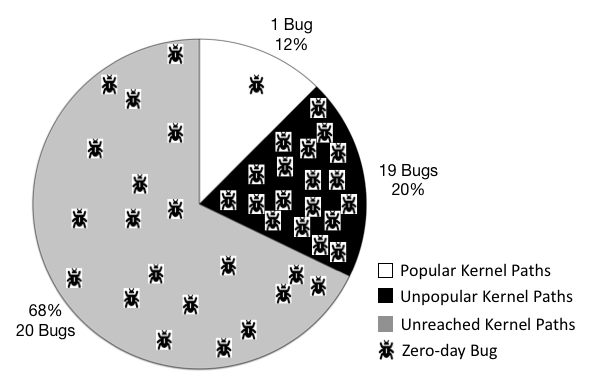
\includegraphics[width=1.0\columnwidth]{diagram/popular_paths.png}
\caption{\small Percentage of different kernel areas that were reached during
 LTP and Trinity system call fuzzing experiments, with the zero-day kernel bugs identified
 in each area.}
\label{fig:coverage}
\end{figure}

%After examining the set of lines that were patched to fix bugs and the traces for
%the commonly-used kernel paths,
\noindent
{\bf Bug distribution.}
The experimental results from Section~\ref{sec-setup} show that only one of the 40 kernel bugs
tested for was found among the popular paths, even though these paths make up 12.4\% of the kernel
(Figure \ref{fig:coverage}).

To test the significance of these results, we performed a power analysis.
%utilizing a Poisson distribution, a form of probability analysis to express the
%likelihood of a given number of events occurring in a fixed interval of time
%and/or space.
%
%Our analysis proceeded as follows.
We assume that kernel bugs appear at an average rate proportional to the
number of lines of kernel code.
%and different kernel parts may have different rates that bugs appear.
%independently of the time since the last bug occurrence.
Therefore, consistent with prior research~\cite{mayer1989probability},
%\yiwen{add more recent citation?}
the rate of defect occurrence per LOC follows a Poisson
distribution~\cite{Poisson-distribution}.
%who proposed a probability model for characterizing the relationship
%between discrete data set.
The premise we tested is that bugs occur at different rates in different
parts of the kernel, i.e., that the less popular kernel portion has more bugs.

We first divided the kernel into two sets,
$A$ and $B$, where bugs occur at rates $\lambda_A$ and
$\lambda_B$, and $\lambda_A \neq \lambda_B$. In this test, $A$ represents the popular
paths in the kernel, while $B$
addresses the less commonly-used paths. Given the null hypothesis
that the rate of defect occurrences is the \textit{same} in set $A$ and $B$
(or bugs in $A$ and $B$ are drawn from the same Poisson distribution),
we used the Uniformly Most Powerful Unbiased (UMPU) test~\cite{shiue1982experiment}
to compare unequal-sized code blocks.
At a significance level of $\alpha=0.01$, the test was significant at
$p=0.0015$, rejecting the null hypothesis.
The test also reported a 95\% confidence that $\lambda_A / \lambda_B
\in [0.002, 0.525]$. This indicates that the ratio between the bug rates is well
below 1. Since $B$ has a bug rate much larger than that of $A$,
%
this result shows that
popular paths have a much lower bug rate than unpopular ones.
%which means that the popular kernel paths
%contain much fewer bugs. Our metric is thus effective in locating bugs in the Linux kernel.


%\cappos{I need to think what to do here.  Perhaps combine into the previous
%section.  We say a lot without saying a lot...}\yanyan{I need to think more..}

\begin{figure}
\centering
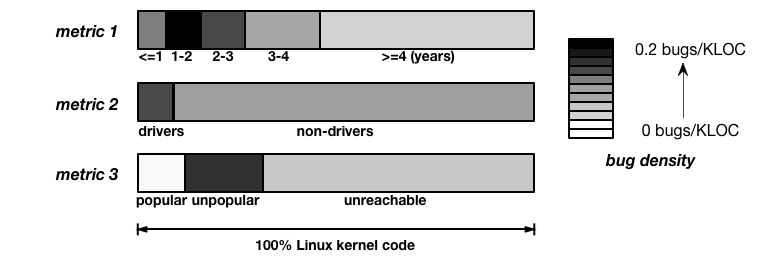
\includegraphics[width=1.1\columnwidth]{diagram/bug_density_v2.png}
\caption{\small Bug density comparison among three metrics.}
\label{fig:bug_density}
\end{figure}

\noindent
{\bf Comparison with other security metrics.}
Ozment, et al.~\cite{ozment2006milk} demonstrated that older code in the
Berkeley Software Distribution (BSD) \cite{BSD}
kernel tended to have fewer bugs (metric 1).
%They determined that a significant extent (61\%) of the reported
%vulnerabilities were
%%``foundational," meaning they were
%introduced prior to the initial version studied.
%They also reported these vulnerabilities have a median lifetime of at least 2.6 years.
To test Ozment's metric using our Linux bug dataset,
we separated the code into five different age groups.
Our results (Figure \ref{fig:bug_density}) showed a substantial
number of bugs located in each group, and not just in the newer code.
%No evident cluster patterns among bugs in any particular age group could be identified.
Therefore, buggy code in the Linux kernel cannot be identified simply
by this age-based metric.
In addition, this metric would seem to have limited use for designing a secure
virtualization system,
%New code is frequently needed to provide additional functionality,
%fix existing problems in the form of patches, and add new technology to improve
%user experience. A
as no system could run very long exclusively on old code.

Another metric, reported by Chou, et al.~\cite{PittSFIeld}, showed that certain parts of the kernel,
particularly device drivers, were more vulnerable than others (metric 2).
%In particular, they identified that device drivers have much more vulnerabilities.
Applying this metric on our dataset, we found that the driver code in our version
of the Linux kernel accounted for only 8.9\% of the total codebase, and contained
just 4 out of the 40 bugs (Figure \ref{fig:bug_density}).
One reason for this is that after Chou's study was published system
designers focused efforts on improving driver code. Palix \cite{palix2011faults}
found that %with development of the Linux kernel,
\texttt{drivers} now has a lower fault rate than other directories,
such as \texttt{arch} and \texttt{fs}.
%However, this metric also proves to be difficult to use with the
%Linux kernel, since our results show that
%only 10.0\% of the kernel bugs could be detected.


%{\bf file vs line granularity}
%Over the years, a number of metrics for identifying bugs in the OS kernel have
%previously been proposed. Most of these
Additionally, there are other security metrics that operate at a coarser granularity,
e.g., the file level. However, when our kernel tests were run at a file
granularity, we found that even popular programs used parts of %as many as
32 files that contained flaws. Yet, only one bug was triggered by those programs.
In addition, common programs tested at this level also executed 36 functions
that were later patched to fix security
flaws, indicating the need to localize bugs at a finer granularity.
%A few researchers have studied metrics at a finer granularity than file level, which
%is at the lines-of-code.
%We now discuss two such metrics, and use our Linux kernel version and 40 bugs dataset
%to conduct a comparison between them and our popular-paths metric.

To summarize, our results demonstrate that previously proposed security
metrics show only weak correlation between the occurrence of bugs
and the type of code they target. In contrast, our metric (metric 3)
provides an effective and statistically significant
%($\alpha=0.01$, $\rho=0.0015$)
means for predicting where in the kernel exploitable flaws
will likely be found. For the remainder of the paper, we will
focus on using our ``popular paths'' metric to design and build secure virtualization systems.

\section{A New Design for Secure Virtualization Systems}
\label{sec.design}

%Providing essential system functionality without exposing privileged code is a
%critical challenge in the design of secure systems.
%Currently, there are two basic approaches.
%One, known as system call interposition (SCI), checks and passes system calls
%through to the underlying kernel. The other, which we call ``functionality
%re-creation," requires rebuilding system functionality with new code. In this
%section, we show that both existing methods are limited in their ability to
%prevent attacks in the kernel.
%Using our metric described in Section~\ref{sec.metric},
%we then propose a new design scheme named \lip, which accesses only popular
%code paths through a very small trusted computing base, and utilizes
%functionality re-creation within a secure sandboxed environment for complex implementations.

In the previous section we have demonstrated that ``popular paths'' correlates statistically-significantly with security. 
Next, we want to demonstrate that our ``popular paths'' metric is practically useful in devising a feasible design solution to build 
secure virtualization systems. We first briefly discuss the limitations faced by existing methods, due to the lack of a good 
security metric. We then discuss our new design scheme named \lip, which comes out of our metric, that accesses only popular code paths. 

\subsection{Previous Attempts and Their Limitations}

\subsubsection{System Call Interposition (SCI)}
SCI systems~\cite{Janus0:96, Janus:99} filter system calls to mediate requests
from untrusted user code instead of allowing it to go directly to the kernel.
The filter checks a predefined security policy to decide which system calls are
allowed to pass to the underlying kernel, and which ones must be stopped.
%Figure \ref{fig:design_system_call_interposition} illustrates how
%system call interposition works. System administrators have direct access to a policy engine that sets and changes security policies.

%\begin{figure}%[h]
%\centering
%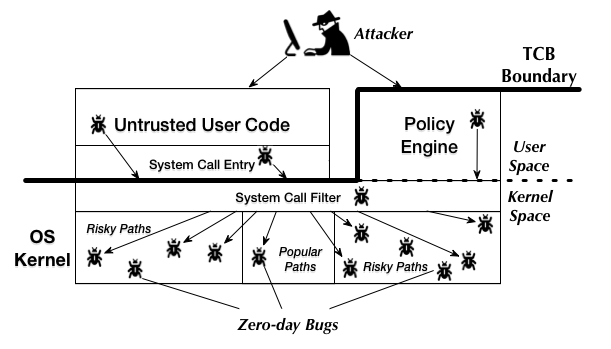
\includegraphics[width=1.0\columnwidth]{diagram/Virtualization_Design_Model_03.png}
%\caption{\small Schematic of how System Call Interposition functions.}
%\label{fig:design_system_call_interposition}
%\end{figure}

%SCI was once popular
%approach to the design of secure virtualization systems because
%because it gave developers the ability to set and enforce security policies.
%\lois{I think I asked this during the last revision. You say ``was"
%a popular approach. Is it not a popular approach anymore?}
%\yiwen{It is not a popular approach anymore, since no modern design could simply rely on
%this idea to build practical system.}
This design is limited by its overly complicated approach to policy
decisions and implementation.
To make a policy decision, the system needs to
obtain and interpret the OS state (e.g., permissions, user groups, register flags)
associated with the programs it is monitoring.
The complexity of OS states makes this process difficult and can lead to
inaccurate policy decisions.
%In addition, there are many indirect paths in the kernel that can be accessed.
%If security policy makers overlook those paths, it renders the
%policy ineffective, as attackers will be able to
%bypass security checks.
%Moreover, blocking
%certain system calls could affect necessary functionality.
%It is difficult for developers to fully understand the side-effects of all the
%system calls in an interface as complex as the UNIX API.
%For example, many applications that rely on \texttt{setuid} fail to check its return value.
%If \texttt{setuid} fails, these applications will continue to function in a compromised state,
%with incorrect permissions and privileges.
%The above limitations make it very challenging to design and build a secure virtualization system using
%system call interposition alone.
%More importantly, there is not a good security metric to indicate if a set of policy decisions is good. 

\subsubsection{Functionality Re-Creation}
Systems such as Drawbridge \cite{Drawbridge-11},
Bascule \cite{Bascule}, and Graphene \cite{Graphene-14} can
provide richer functionality and run more complex programs than most systems built
with SCI alone because they have their own
interfaces and libraries. We label such a design
as ``functionality re-creation."

%\begin{figure}%[h]
%\centering
%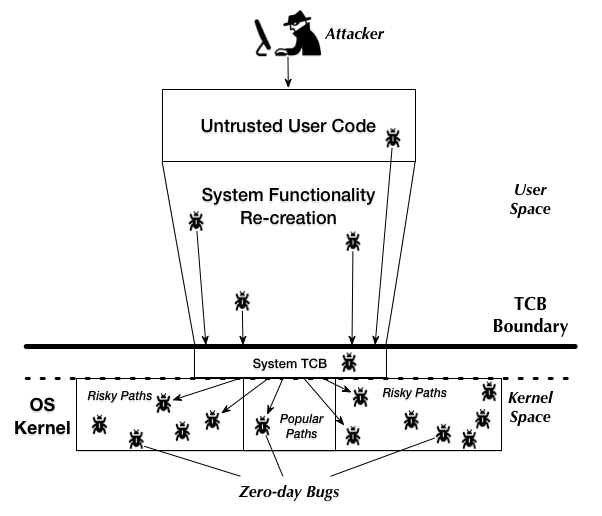
\includegraphics[width=1.0\columnwidth]{diagram/Virtualization_Design_Model_02.png}
%\caption{\small Schematic of a Functionality Re-creation System.}
%\label{fig:design_functionality_reimplementation}
%\end{figure}

The key to this design is to not fully rely on the underlying
kernel for system functions. 
%As illustrated in Figure \ref{fig:design_functionality_reimplementation},
This design re-creates its own system functionalities to provide to user code.
When it has to %communicate with the kernel to
access resources like memory, CPU, and disk storage, the system accesses the kernel directly with
its underlying TCB code.
%which can access the kernel directly.
%For example, Graphene \cite{Graphene-14} re-creates its own Linux system calls
%in \texttt{libLinux.so}. When it needs to acquire resources from the kernel, it
%uses a Platform Adaptation Layer (PAL) with access to the kernel, and provides
%basic API functions to the OS library.

Functionality re-creation provides a more realistic solution to building
virtualization systems than earlier efforts.
However, functionality re-creation has two pitfalls: 
first, if the re-created functionality resides in the TCB of the virtualization system, then vulnerabilities there can expose the host OS to attack as well.
For example, hundreds of vulnerabilities have been
reported in existing virtualization systems such as QEMU and VMWare over the past ten years~\cite{NVD}.
%In addition, the
%complex semantics of OS functions can easily lead to the emergence of bugs during
%the re-creation process. Some of these vulnerabilities
%can directly lead to privilege escalation, which allows attackers to escape the sandbox
%and execute arbitrary code on the host OS.
%For example, a vulnerability in VMWare's codebase caused by buffer overflows in the VIX
%API allowed local users to
%gain privilege to execute arbitrary code in the host
%OS~\cite{CVE-2008-2100}.

Second, functionality re-creation may assume that the underlying host kernel is correct. 
As we have seen, this assumption is often incorrect; host kernels may have bugs in their implementation that leave them vulnerable to attack. 
Thus, to provide the greatest assurance that the host kernel will not be exposed to malicious user programs, 
a secure functionality re-creation design should try to deliberately avoid kernel paths that are likely to contain flaws. 
We discuss this approach in detail next.

\subsection{Lock-in-Pop: Staying on the Beaten Path}
\label{lock-in-pop}

%As discussed above, a weakness of the previous approaches is the inevitable contact
%between the privileged kernel code and an untrusted application.
Recall that we want to show that the ``popular paths'' metric can be used in practice. 
We do so by leveraging this ``popular kernel paths '' metric, which contain fewer bugs, to devise a design
in which all code, including the complex part
of the operating system interface, access only
``popular kernel paths'' through a small TCB. As it ``locks" all functionality
requests into only the ``popular paths'', we dubbed the design \lip.

\begin{figure}%[h]
\centering
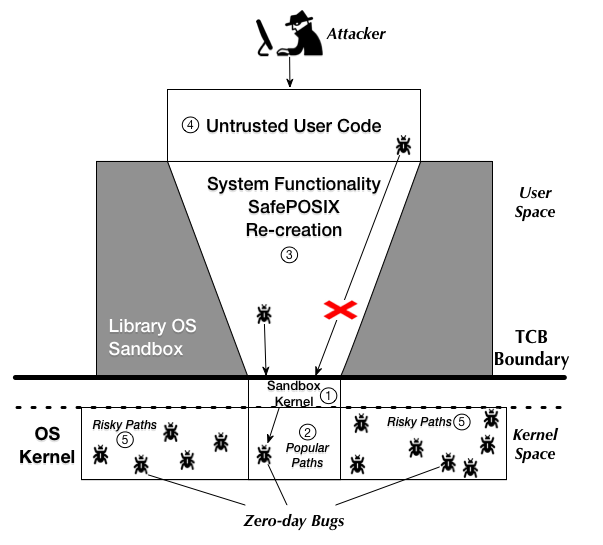
\includegraphics[width=1.0\columnwidth]{diagram/Virtualization_Design_Model_01.png}
\caption{\small \lip design ensures safe execution of untrusted user code
despite existing potential zero-day bugs in the OS kernel.}
\label{fig:design_safe_reimplementation}
\end{figure}

At the lowest level of the design (interfacing with the host OS) is the
sandbox kernel (\ding{172} in Figure \ref{fig:design_safe_reimplementation}).
The sandbox kernel's main role is to ensure that only popular paths (\ding{173} in Figure \ref{fig:design_safe_reimplementation})
of the host OS's kernel can be accessed. 
The sandbox kernel could thus function as a very granular system call filter, or
as the core of a programming language sandbox. Note that the functionality
provided by the sandbox kernel is (intentionally) much less than what
an application needs. For example, an application may store files in directories and set permissions on those files.
The sandbox kernel may provide a much simpler abstraction (e.g., a block storage abstraction),
so long as the strictly needed functionality (e.g., persistent storage) is provided.

In our \lip design, a key component is the sandbox kernel (\ding{172} in Figure \ref{fig:design_safe_reimplementation}), 
which controls access to the underlying host kernel. 
Constructing the sandbox kernel is not dependent on any specific technique or programming language. 
Instead, the sandbox kernel follows a central design principle to include only simple and necessary system calls with basic flags, 
which can be checked to verify that only ``popular paths'' were used.  
The sandbox kernel should start with building-block functions to first form a minimum set of system calls. 
To give one example, for network programs, opening a TCP connection would be considered an essential function. 
So, we would check that lines of kernel code, such as lines in \texttt{void tcp\_init\_sock(struct sock *sk)}, that correspond 
with opening TCP sockets, were included in ``popular paths'' for that system, and the \texttt{open\_tcp\_connection()} function 
would be included in the sandbox kernel. 
Examples of other necessary functions are \texttt{file.open, file.close, file.read, file.write} for file system 
functions, and \texttt{create\_thread, create\_lock, lock.acquire, lock.release} for threading functions. 

In order to make security our priority, the designed sandbox kernel should use only a subset of the ``popular paths''. 
For systems where security is not as critical, trade-offs can certainly be made to include some ``unpopular paths'' to accommodate applications. 
Further discussion of this trade-off is beyond the scope of this paper, 
though we acknowledge it is an issue that should be addressed as \lip is deployed. 
While restricting the system call interface is a big hammer for limiting access to ``popular paths'' in the kernel, 
we believe that this is the best choice available, given that we do not want to require modification to the kernel, and 
would like to allow users to easily run their applications without much extra effort. 

The application is provided more complex functionality due to the SafePOSIX re-creation
(\ding{174} in Figure \ref{fig:design_safe_reimplementation}).
SafePOSIX has the needed complexity to build the more convenient higher-level
abstractions using the basic functionality the sandbox kernel provides.
The SafePOSIX re-creation is itself isolated within a library OS sandbox, which
forces all system calls to go through the sandbox kernel.
So long as this is performed, all calls from SafePOSIX re-creation will only touch the permitted (popular) kernel paths in the underlying host OS.

Similarly, untrusted user code (\ding{175} in Figure \ref{fig:design_safe_reimplementation}) also must be restricted in the way
in which it performs system calls.
System calls must go through the SafePOSIX re-creation, into the sandbox kernel, and then to the host OS.
This is done because if user code could directly make system calls, it could access any paths in the host OS's kernel desired
and thus exploit bugs within them.

Note that it is expected that bugs will occur in many components.
We expect that bugs will occur in the non-popular (risky) kernel paths (\ding{176} in Figure \ref{fig:design_safe_reimplementation}),
bugs will exist in the SafePOSIX re-creation, and the user program will be buggy or even explicitly malicious (created by attackers).
Since the remaining components (\ding{172} and \ding{173} in Figure \ref{fig:design_safe_reimplementation})
are small and/or well tested, this leads to a lower risk of compromise.

\subsection{Implementation of Lock-in-Pop}
\label{implementation}

To test the practicality of the ``popular paths'' metric and our \lip design, 
we implement a prototype virtual machine
called Lind\footnote{\scriptsize Lind is an old English word for a lightweight, but still strong shield
constructed from two layers of linden wood.}. The purpose of building the Lind prototype is to demonstrate that 
our ``popular paths'' metric is practical. And it is indeed possible for developers to build secure systems using 
``popular paths''. 
Lind is divided into a \emph{computational module} that enforces software fault isolation (SFI) and a
\emph{SafePOSIX module} that safely re-creates OS functionality needed by user
applications.  We use a slightly modified version of Native Client
(NaCl)~\cite{NaCl-09} for the computational module; the SafePOSIX is
implemented using Restricted Python (Repy)~\cite{Repy-10}, to support
complex user applications without exposing potentially risky kernel paths.

In this section we provide a brief description of these components and how they
were integrated into Lind, followed by an example of how the system works.

\subsubsection{Primary Components}

\paragraph{Native Client.}
We use NaCl to isolate the computation of the user application
from the kernel. NaCl allows Lind to work on most types of legacy code.
It compiles the programs to produce a binary with software fault isolation.
This prevents applications from performing system calls
or executing arbitrary instructions.
Instead, the application will call into a small, privileged
part of NaCl that forwards system calls. In NaCl's original implementation,
these calls would usually be forwarded to the host OS kernel. In Lind, we
modified NaCl to instead forward these calls to our SafePOSIX re-creation 
(described in detail below).

\paragraph{SafePOSIX.}

To build an API that can access the safe parts of the underlying kernel while
still supporting existing applications, we need two things. First, we need a
restricted sandbox kernel that only allows access to popular kernel paths. We
used Seattle's Repy~\cite{Repy-10} sandbox to perform this task. Second, we
have to provide complex system functions to user programs,
for which we implemented the widely accepted standard POSIX interface on top of Repy, 
which we call SafePOSIX. 

Because the sandbox kernel is the only code that will be in direct contact with host
system calls, it should be small (to make it easy to audit), while providing
primitives that can be used to build more complex functionality.
We used Seattle's Repy system API due to its tiny (around 8K LOC) sandbox
kernel, and its minimal set of system call APIs needed to build general
computational functionality. Repy allows access only to the popular portions of
the OS kernel through 33 basic API functions, including 13 network functions, 6
file functions, 6 threading functions, and 8 miscellaneous functions (Table
\ref{table:RepyKernel})~\cite{Repy-10, RepyKernel}. 

Repy is only one possible implementation of the sandbox kernel built for our \lip design. 
It was chosen because it starts with basic building-block functions and tries to be conservative. 
Repy was designed and implemented before our ``popular paths'' study, and so it was not a perfect match, 
but it was verified as using only part of the ``popular paths.'' 
As reported in our evaluation (Section~{{\ref{Reachable-Kernel-Trace-Analysis-for-Repy-Sandbox}}), 
Repy accessed a subset (around 70\% to 80\%) of the ``popular paths.'' 

Our current implementation does not end up using all of the ``popular paths''. 
It is certainly safe to use fewer paths than are available, but it is possible that we are missing out on some performance or compatibility gains. 
As we extend our prototype, the ``popular path'' metric will allow us to check whether new APIs we add 
expose potentially unsafe kernel code to applications in the sandbox.

\begin{table}
\centering
  \begin{tabular}{ | p{2.5cm} | p{4.5cm} |}
  \hline
  \textbf{Repy Function} & \textbf{Available System Calls}  \\ \hline

Networking & \emph{gethostbyname, openconnection, getmyip, socket.send, socket.receive, socket.close,
listenforconnection, tcpserversocket.getconnection, tcpserversocket.close, sendmessage, listenformessage,
udpserversocket.getmessage, and udpserversocket.close.} \\ \hline

File System I/O Operations & \emph{openfile(filename, create), file.close(), file.readat(size limit, offset), file.writeat(data, offset),
listfiles(), and removefile(filename).} \\ \hline

Threading & \emph{createlock, sleep, lock.acquire, lock.release, createthread, and getthreadname.} \\ \hline

Miscellaneous Functions & \emph{getruntime, randombytes, log, exitall, createvirtualnamespace,
virtualnamespace.evaluate, getresources, and getlasterror.}  \\ \hline
    \end{tabular}
    \caption{Repy sandbox kernel functions that support Lind's SafePOSIX re-creation.}
    \label{table:RepyKernel}
\end{table}


\subsubsection{Enhanced Safety in Call Handling with SafePOSIX Re-creation}

The full kernel interface is extremely rich and hard to protect.
The dual sandbox \lip design used to build Lind provides enhanced
safety protection through both isolation and a POSIX interface (SafePOSIX) that
re-creates risky system calls to
provide full-featured API for legacy applications, with minimal impact on the kernel.

In Lind, a system call issued from user code is
received by NaCl, and then redirected to SafePOSIX.
To service a system call in NaCl, a server routine in
Lind marshals its arguments into a text string, and sends the call and the arguments
to SafePOSIX. The SafePOSIX re-creation serves the system call request, marshals the result, and
returns it back to NaCl. Eventually, the result is returned as the appropriate
native type to the calling program.

SafePOSIX is safe because of two design principles.
First, its re-creation only relies on a small set of basic Repy functions (Table \ref{table:RepyKernel}).
Therefore, the interaction with the host OS kernel is strictly controlled.
Second, the SafePOSIX re-creation is run within the Repy programming language sandbox,
which properly isolates any bugs inside SafePOSIX itself.

%We now offer a more detailed example of how SafePOSIX works by reviewing how it re-creates a file system. 
%The core of the SafePOSIX file system is the \texttt{open}, \texttt{close}, \texttt{read}, \texttt{write},
%\texttt{getdents}, \texttt{stat}, \texttt{mkdir} and \texttt{rmdir} system calls.
%These give the program the illusion of a normal file system even though Repy does not allow directories or access to file attributes.

%When Lind starts, the file system does some pre-initialization. Using the Repy API, the SafePOSIX file system reads a file named ``lind.metadata''
%from the local directory. This file contains packed metadata from previous runs of Lind,
%and is loaded into the runtime SafePOSIX file system data structures.
%There are three main data structures: a list of open file handles, a Python dict of inodes and file metadata,
%and a mapping table to go from a file name and path to an inode number.
%All these data structures are stored in memory, and written to disk when they are changed.

%The \texttt{open} system call is the normal starting point for most file system operations.
%Given a path, it will return a file descriptor to perform other operations like \texttt{read} and \texttt{write}.
%When SafePOSIX receives the \texttt{open} system call, it parses the path, and
%traverses the path in the inode lookup table.
%When SafePOSIX finds the file, it uses the Repy \texttt{openfile} call to get the backing file's object.
%It then picks a free entry from the file handle table, and stores a link to the inode and the file object.
%If the \texttt{create} flag is passed, it adds an entry to the inode and inode lookup table, and creates a new backing file.
%The backing files are not named the same as the actual files, but rather just ``linddata.001,'' ``linddata.002,'' etc.
%The simple names for the backing files allow us to store the real file name in the metadata, a
%necessary step because of Repy's strict rules about the content of filenames.
%Finally, the call returns the index into the file handle table or, if an error was encountered, an error number to which the Unix \texttt{errno} value is set.

%Here is another example of how SafePOSIX re-creation would work with the symbolic link function.
%Instead of relying on the underlying kernel to create symbolic links between real files
%in the host file system, SafePOSIX builds and maintains its own metadata to represent a virtual symbolic link
%between files within its system. In this case, if there is a bug in this symbolic link function,
%such as creation of a link with a deleted file, the bug will be contained within the SafePOSIX re-creation.
%As a result, instead of creating a security issue, the application is denied privileged access to the host OS kernel.
%Therefore, attackers will not be able to leverage a bug within the symbolic link function to exploit the host kernel.

%As described in the above example, the SafePOSIX re-creation only uses a few Repy sandbox kernel functions to access the hardware.
%It creates and maintains its own metadata and data structures, using the Repy programming language sandbox.
%\section{Implementation of Lind}
\label{sec.implementation}

To test our \lip design, we used it to implement a secure virtual machine
called Lind\footnote{\scriptsize Lind is an old English word for a lightweight, but still strong shield
constructed from two layers of linden wood.}. Lind is divided into a
\emph{computational module} that enforces software fault isolation (SFI) and a
\emph{SafePOSIX module} that safely re-creates OS functionality needed by user
applications. We use a slightly modified version of Native Client
(NaCl)~\cite{NaCl-09} for the computational module; the SafePOSIX is
implemented using Restricted Python (Repy)~\cite{Repy-10}, to support
complex user applications without exposing potentially risky kernel paths.

In this section we provide a brief description of these components and how they
were integrated into Lind, followed by an example of how the system works.

\subsection{Primary Components}

\paragraph{Native Client.}
We use NaCl to isolate the computation of the user application
from the kernel. NaCl allows Lind to work on most types of legacy code.
It compiles the programs to produce a binary with software fault isolation.
This prevents applications from performing system calls
or executing arbitrary instructions.
Instead, the application will call into a small, privileged
part of NaCl that forwards system calls. In NaCl's original implementation,
these calls would usually be forwarded to the host OS kernel. In Lind, we
modified NaCl to instead forward these calls to our SafePOSIX re-creation 
(described in detail below).

\paragraph{SafePOSIX.}

To build an API that can access the safe parts of the underlying kernel while
still supporting existing applications, we need two things. First, we need a
restricted sandbox that only allows access to commonly-used kernel paths. We
used Seattle's Repy~\cite{Repy-10} sandbox to perform this task. Second, we
have to provide complex system functions to user programs,
for which we implemented the widely accepted standard POSIX interface on top of Repy, 
which we call SafePOSIX. 

Because the sandbox kernel is the only code that will be in direct contact with host
system calls, it should be small (to make it easy to audit), while providing
primitives that can be used to build more complex functionality.
We used Seattle's Repy system API due to its tiny (around 8K LOC) sandbox
kernel, and its minimal set of system call APIs needed to build general
computational functionality. Repy allows access only to the popular portions of
the OS kernel through 33 basic API functions, including 13 network functions, 6
file functions, 6 threading functions, and 8 miscellaneous functions (Table
\ref{table:RepyKernel})~\cite{Repy-10, RepyKernel}.

\begin{table}
\centering
  \begin{tabular}{ | p{2.5cm} | p{4.5cm} |}
  \hline
  \textbf{Repy Function} & \textbf{Available System Calls}  \\ \hline

Networking & \emph{gethostbyname, openconnection, getmyip, socket.send, socket.receive, socket.close,
listenforconnection, tcpserversocket.getconnection, tcpserversocket.close, sendmessage, listenformessage,
udpserversocket.getmessage, and udpserversocket.close.} \\ \hline

File System I/O Operations & \emph{openfile(filename, create), file.close(), file.readat(size limit, offset), file.writeat(data, offset),
listfiles(), and removefile(filename).} \\ \hline

Threading & \emph{createlock, sleep, lock.acquire, lock.release, createthread, and getthreadname.} \\ \hline

Miscellaneous Functions & \emph{getruntime, randombytes, log, exitall, createvirtualnamespace,
virtualnamespace.evaluate, getresources, and getlasterror.}  \\ \hline
    \end{tabular}
    \caption{Repy sandbox kernel functions that support Lind's SafePOSIX re-creation.}
    \label{table:RepyKernel}
\end{table}


\subsection{Enhanced Safety in Call Handling with SafePOSIX Re-creation}

The full kernel interface is extremely rich and hard to protect.
The dual sandbox \lip design used to build Lind provides enhanced
safety protection through both isolation and a POSIX interface (SafePOSIX) that
re-creates risky system calls to
provide full-featured API for legacy applications, with minimal impact on the kernel.

In Lind, a system call issued from user code is
received by NaCl, and then redirected to SafePOSIX.
To service a system call in NaCl, a server routine in
Lind marshals its arguments into a text string, and sends the call and the arguments
to SafePOSIX. The SafePOSIX re-creation serves the system call request, marshals the result, and
returns it back to NaCl. Eventually, the result is returned as the appropriate
native type to the calling program.

SafePOSIX is safe because of two design principles.
First, its re-creation only relies on a small set of basic Repy functions (Table \ref{table:RepyKernel}).
Therefore, the interaction with the host OS kernel is strictly controlled.
Second, the SafePOSIX re-creation is run within the Repy programming language sandbox,
which properly isolates any bugs inside SafePOSIX itself.

We now offer a more detailed example of how SafePOSIX works by reviewing how it re-creates a file system. 
The core of the SafePOSIX file system is the \texttt{open}, \texttt{close}, \texttt{read}, \texttt{write},
\texttt{getdents}, \texttt{stat}, \texttt{mkdir} and \texttt{rmdir} system calls.
These give the program the illusion of a normal file system even though Repy does not allow directories or access to file attributes.

When Lind starts, the file system does some pre-initialization. Using the Repy API, the SafePOSIX file system reads a file named ``lind.metadata''
from the local directory. This file contains packed metadata from previous runs of Lind,
and is loaded into the runtime SafePOSIX file system data structures.
%There are three main data structures: a list of open file handles, a Python dict of inodes and file metadata,
%and a mapping table to go from a file name and path to an inode number.
%All these data structures are stored in memory, and written to disk when they are changed.

The \texttt{open} system call is the normal starting point for most file system operations.
Given a path, it will return a file descriptor to perform other operations like \texttt{read} and \texttt{write}.
When SafePOSIX receives the \texttt{open} system call, it parses the path, and
traverses the path in the inode lookup table.
When SafePOSIX finds the file, it uses the Repy \texttt{openfile} call to get the backing file's object.
It then picks a free entry from the file handle table, and stores a link to the inode and the file object.
If the \texttt{create} flag is passed, it adds an entry to the inode and inode lookup table, and creates a new backing file.
The backing files are not named the same as the actual files, but rather just ``linddata.001,'' ``linddata.002,'' etc.
The simple names for the backing files allow us to store the real file name in the metadata, a
necessary step because of Repy's strict rules about the content of filenames.
%Finally, the call returns the index into the file handle table or, if an error was encountered, an error number to which the Unix \texttt{errno} value is set.

%Here is another example of how SafePOSIX re-creation would work with the symbolic link function.
%Instead of relying on the underlying kernel to create symbolic links between real files
%in the host file system, SafePOSIX builds and maintains its own metadata to represent a virtual symbolic link
%between files within its system. In this case, if there is a bug in this symbolic link function,
%such as creation of a link with a deleted file, the bug will be contained within the SafePOSIX re-creation.
%As a result, instead of creating a security issue, the application is denied privileged access to the host OS kernel.
%Therefore, attackers will not be able to leverage a bug within the symbolic link function to exploit the host kernel.

As described in the above example, the SafePOSIX re-creation only uses a few Repy sandbox kernel functions to access the hardware.
It creates and maintains its own metadata and data structures, using the Repy programming language sandbox.

\section{Evaluation}
\label{sec.evaluation}

To demonstrate that our ``popular paths'' metric is useful and practical,
we use our Lind prototype as a testing tool.
%in containing untrusted code and protecting the OS kernel,
We compared Lind against three existing
virtualization systems -- Docker, LXC, and Graphene.
%This section describes
%the purpose and setup of our experiments, and presents and discusses our results.
We chose these three systems because they currently represent the most
widely-used VM design models for securing the OS kernel.
LXC is a well-known container designed specifically for the Linux kernel.
Docker is a widely-used container that wraps an application in a self-contained filesystem, while
Graphene is an open source library OS designed to run an application in a virtual machine environment.
Lastly, we also tested Native Linux to serve as a
baseline for comparison.
%
Our tests were designed to answer four fundamental questions:

\textit{How does Lind compare to other virtualization systems
in protecting against zero-day Linux kernel bugs?}
(Section~{\ref{Linux-Kernel-Bug-Test-and-Evaluation}})

\textit{How much of the underlying kernel code is exposed, and is thus
vulnerable in different virtualization systems?}
(Section~{{\ref{Reachable-Kernel-Trace-Analysis-for-Different-Virtualization-Systems}})

\textit{If Lind's SafePOSIX construction has bugs, how severe an impact would
this vulnerability have?}
(Section~{{\ref{Reachable-Kernel-Trace-Analysis-for-Repy-Sandbox}})

\textit{In the Lind prototype, what would be the expected performance overhead in
real-world applications? Can developers make use of the ``popular paths'' metric to develop
practical systems?}
(Section~{{\ref{Performance-Evaluation}})

\subsection{Linux Kernel Bug Test and Evaluation}
\label{Linux-Kernel-Bug-Test-and-Evaluation}

%\textbf{Test Purpose.}
%To evaluate how well each virtualization system protects the Linux kernel
%against reported zero-day bugs.
%\brendan{This is my best understanding of how the tests were conducted. Yiwen et al., please jump in and correct me if I got something wrong.}
%\yiwen{The setup section looks good to me.}

\noindent
\textbf{Setup.}
To evaluate how well each virtualization system protects the Linux kernel
against reported zero-day bugs,
we examined a list of 69 historical bugs that had been identified and patched in
versions 3.13.0 and 3.14.1 of the Linux kernel \cite{CVE-Datasource}.
By consulting the National Vulnerability Database (NVD) \cite{NVD}, we obtained
a list of all CVEs \cite{CVE} that were known to exist in these Linux kernel
versions as of September 2015; we found 69 such vulnerabilities.
By analyzing security patches for those bugs,
we were able to identify the lines of code in the kernel that correspond to each one.

In the following evaluation, we assume that a bug is potentially triggerable if the lines of code that were changed in the patch are reached
(i.e., the same metric described in Section~\ref{sec.metric}).
This measure may overestimate potential danger posed by a system since simply reaching the buggy code does not mean that guest code
actually has enough control to exploit the bug.
However, this overestimate should apply equally to all of the systems we tested, which means it is still a useful method of comparison.

Next, we sought out proof-of-concept code that could trigger each bug.
We were able to obtain or create code to trigger nine out of the 69 bugs \cite{Exploit-Database}.
For the rest, we used the Trinity system call fuzzer
\cite{Trinity} on Linux 3.14.1 (referred to as ``Native'' Linux in Table~\ref{table:trigger_vulnerabilities}).
By comparing the code reached during fuzzing with the lines of code affected by security patches,
we were able to identify an additional 26 bugs that could be triggered.
All together, we identified a total of 35 bugs that we were able to trigger from the user space, and these formed our final dataset for the evaluation.

We then evaluated the protection afforded by four virtualization systems (including Lind) by attempting to trigger the 35 bugs from inside each one.
The host system for each test ran a version of Linux 3.14.1 with gcov instrumentation enabled.
For the nine bugs that we could trigger directly, we ran the proof of concept exploit inside the guest.
For the other 26, we ran the Trinity fuzzer inside the guest, exercising each system call 1,000,000 times with random inputs.
Finally, we checked whether the lines of code containing each bug were reached in the host kernel,
indicating that the guest could have triggered the bug.

\noindent
\textbf{Results.}
We found that a substantial number of bugs could be triggered in existing
virtualization systems, as shown in Table \ref{table:trigger_vulnerabilities}.
All (100\%) bugs were triggered in Native Linux,
while the other programs had lower rates: 8/35 (22.9\%)  in Docker,
12/35 (34.3\%)  in LXC, and 8/35 (22.9\%) bugs in Graphene.
In comparison, only 1 out of 35 bugs  (2.9\%) was triggered in Lind.

When we take a closer look at the results, we can see that these outcomes
have a lot to do with the design principles of the virtualization systems and
the way in which they handle system call requests.
Graphene \cite{Graphene-14} is a library OS that relies heavily on the Linux kernel to handle system calls.
Graphene's Linux library implements the Linux system calls using a variant of the
Drawbridge \cite{Drawbridge-11} ABI, which has 43 functions. Those ABI functions
are provided by the Platform Adaptation Layer (PAL), implemented using 50 calls
to the kernel. It turns out that 8 vulnerabilities in our test were triggered by PAL's
50 system calls. On the contrary, Lind only relies on 33 system calls, which
significantly reduces risk and avoids 7 out of the 8 bugs.

Graphene supports many complex and risky system calls, such as \texttt{execve}, \texttt{msgsnd}, and \texttt{futex},
that reached the risky (unpopular) portion of the kernel and eventually led to kernel bugs.
In addition, for many basic and frequently-used system calls like \texttt{open} and \texttt{read},
Graphene allows rarely-used flags and arguments to be passed down to the kernel, which triggered bugs in
the unpopular paths.
In Lind, all system calls only allow a restricted set of simple and frequently-used flags and arguments.
One example from our test result is that Graphene allows \texttt{O\_TMPFILE} flag to pass down with
\texttt{path\_openat()} system call. This reached risky lines of code inside \texttt{fs/namei.c} in the kernel,
and eventually triggered bug CVE-2015-5706.
The same bug was triggered in the same way inside Docker and LXC, but was successfully prevented by Lind,
due to its strict control of flags and arguments.
In fact, the design of Graphene requires extensive interaction
with the host kernel and, hence, has many risks. The developers of Graphene manually conducted
an analysis of 291 Linux vulnerabilities from 2011 to 2013, and found out that Graphene's design can not prevent 144 of those vulnerabilities.

LXC \cite{LXC} is an operating-system-level virtualization container that uses Linux kernel features to achieve containment.
Docker \cite{Docker} is a Linux container that runs on top of LXC. The two containers have very similar design features
that both rely directly on the Linux kernel to handle system call requests. Since system calls inside Docker are passed down
to LXC and then into the kernel, we found out that all 8 kernel vulnerabilities triggered inside Docker were also triggered
with LXC. In addition, LXC interacts with the kernel via its \texttt{liblxc} library component, which triggered the extra 4 bugs.

It should be noted that, although the design of Lind only accesses popular paths in the kernel and implements SafePOSIX inside
of a sandbox, there are a few fundamental building blocks for which Lind must rely on the kernel. To be more specific,
\texttt{mmap} and \texttt{threads} cannot be recreated inside SafePOSIX without interaction with the kernel, since there has
to be some basic operations to access the hardware. Therefore, in our design of Lind, \texttt{mmap} and \texttt{threads}
are passed down to the kernel, and any vulnerabilities related to them are  unavoidable.
CVE-2014-4171 is a bug triggered by \texttt{mmap} inside Lind. It was also triggered inside Docker, LXC, and Graphene, indicating
that those systems rely on the kernel to perform \texttt{mmap} operations as well.

Our initial results suggest that bugs are usually triggered by extensive interaction with the unpopular paths in the kernel through
complex system calls, or basic system calls
with complicated or rarely used flags. The \emph{Lock-in-Pop} design, and thus Lind,
provides strictly controlled access to the kernel, and so, poses
the least risk.

%To test if a bug could be triggered, we created or located C
%code capable of exploiting each kernel bug \cite{Exploit-Database}.
%We were only able to trigger and obtain results for 35 out of the 69 bugs in our
%experiments. In some cases, there was a
%difficulty in clearly determining if triggering had occurred, while in other we
%were unable to find code to trigger them. We decided to focus our study on
%this group of 35 bugs and leave the more complex ones to future work.

%We compiled and ran the exploit C code under each virtualization system to
%obtain their kernel traces, and then used our kernel trace safety metric to
%determine if a specific bug was triggered.

%\begin{table*}[!ht]
%\begin{table}[tbp]
%\scriptsize
\begin{table}[h]
\scriptsize
\centering

\begin{tabular}{|p{1.7cm}|p{.6cm}|p{.65cm}|p{.65cm}|p{.9cm}|p{.6cm}|}\hline

\multirow{2}{1.7cm}{\bf Vulnerability}    &  \multirow{2}{.6cm}{\bf Native Linux}
 & \multirow{2}{.6cm}{\bf Docker} & \multirow{2}{.6cm}{\bf LXC} &
\multirow{2}{1cm}{\bf Graphene} & \multirow{2}{.6cm}{\bf Lind} \\
& & & & & \\
\hline

 CVE-2015-5706 & \multirow{1}{.7cm}{{\color{red}\ding{51}}} &
 \multirow{1}{1cm}{{\color{red}\ding{51}}} &
\multirow{1}{1cm}{{\color{red}\ding{51}}} &
\multirow{1}{1cm}{{\color{red}\ding{51}}} &
\ding{55}  \\

 CVE-2015-0239 & \multirow{1}{.7cm}{{\color{red}\ding{51}}} &
 \ding{55} & \multirow{1}{1cm}{{\color{red}\ding{51}}} &
 \ding{55}  & \ding{55}  \\

 CVE-2014-9584 & \multirow{1}{.7cm}{{\color{red}\ding{51}}} &
 \ding{55} & \ding{55} &
 \ding{55}  & \ding{55}  \\

 CVE-2014-9529 & \multirow{1}{.7cm}{{\color{red}\ding{51}}} &
 \ding{55} & \multirow{1}{1cm}{{\color{red}\ding{51}}} &
\ding{55}  & \ding{55}  \\

 CVE-2014-9322 & \multirow{1}{.7cm}{{\color{red}\ding{51}}} &
\multirow{1}{1cm}{{\color{red}\ding{51}}} & \multirow{1}{1cm}{{\color{red}\ding{51}}} &
\multirow{1}{1cm}{{\color{red}\ding{51}}}  & \ding{55}
\\

 CVE-2014-9090 & \multirow{1}{.7cm}{{\color{red}\ding{51}}} &
 \ding{55} & \ding{55} &
 \ding{55}  & \ding{55}  \\

 CVE-2014-8989 & \multirow{1}{.7cm}{{\color{red}\ding{51}}} &
 \multirow{1}{1cm}{{\color{red}\ding{51}}} &
\multirow{1}{1cm}{{\color{red}\ding{51}}} &
\multirow{1}{1cm}{{\color{red}\ding{51}}} &
\ding{55}  \\

 CVE-2014-8559 & \multirow{1}{.7cm}{{\color{red}\ding{51}}} &
 \ding{55} & \ding{55} &
 \ding{55}  & \ding{55}  \\

 CVE-2014-8369 & \multirow{1}{.7cm}{{\color{red}\ding{51}}} &
 \ding{55} & \ding{55} &
 \ding{55}  & \ding{55}  \\

 CVE-2014-8160 & \multirow{1}{.7cm}{{\color{red}\ding{51}}} &
 \ding{55} & \multirow{1}{1cm}{{\color{red}\ding{51}}} &
\ding{55}  & \ding{55}  \\

 CVE-2014-8134 & \multirow{1}{.7cm}{{\color{red}\ding{51}}} &
 \ding{55} & \multirow{1}{1cm}{{\color{red}\ding{51}}} &
\multirow{1}{1cm}{{\color{red}\ding{51}}}  & \ding{55}
\\

 CVE-2014-8133 & \multirow{1}{.7cm}{{\color{red}\ding{51}}} &
 \ding{55} & \ding{55} &
\ding{55}  & \ding{55}  \\

 CVE-2014-8086 & \multirow{1}{.7cm}{{\color{red}\ding{51}}} &
 \multirow{1}{1cm}{{\color{red}\ding{51}}} &
\multirow{1}{1cm}{{\color{red}\ding{51}}} &
\ding{55} & \ding{55}  \\

 CVE-2014-7975 & \multirow{1}{.7cm}{{\color{red}\ding{51}}} &
 \ding{55} & \ding{55} &
 \ding{55}  & \ding{55}  \\

 CVE-2014-7970 & \multirow{1}{.7cm}{{\color{red}\ding{51}}} &
 \ding{55} & \ding{55} &
 \ding{55}  & \ding{55}  \\

 CVE-2014-7842 & \multirow{1}{.7cm}{{\color{red}\ding{51}}} &
 \ding{55} & \ding{55} &
 \ding{55}  & \ding{55}  \\

 CVE-2014-7826 & \multirow{1}{.7cm}{{\color{red}\ding{51}}} &
 \ding{55} & \ding{55}  &
\multirow{1}{1cm}{{\color{red}\ding{51}}}  & \ding{55}
\\

 CVE-2014-7825 & \multirow{1}{.7cm}{{\color{red}\ding{51}}} &
 \ding{55} & \ding{55} &
\multirow{1}{1cm}{{\color{red}\ding{51}}}  & \ding{55}
\\

 CVE-2014-7283 & \multirow{1}{.7cm}{{\color{red}\ding{51}}} &
 \ding{55} & \ding{55} &
 \ding{55}  & \ding{55}  \\

 CVE-2014-5207 & \multirow{1}{.7cm}{{\color{red}\ding{51}}} &
 \ding{55} & \ding{55} &
 \ding{55}  & \ding{55}  \\

 CVE-2014-5206 & \multirow{1}{.7cm}{{\color{red}\ding{51}}} &
 \multirow{1}{1cm}{{\color{red}\ding{51}}} &
\multirow{1}{1cm}{{\color{red}\ding{51}}} &
\ding{55}  & \ding{55}
\\

 CVE-2014-5045 & \multirow{1}{.7cm}{{\color{red}\ding{51}}} &
 \ding{55} & \ding{55} &
 \ding{55}  & \ding{55}  \\

 CVE-2014-4943 & \multirow{1}{.7cm}{{\color{red}\ding{51}}} &
 \ding{55} & \ding{55} &
 \ding{55}  & \ding{55}  \\

 CVE-2014-4667 & \multirow{1}{.7cm}{{\color{red}\ding{51}}} &
 \ding{55} & \ding{55} &
 \multirow{1}{1cm}{{\color{red}\ding{51}}}  & \ding{55}  \\

 CVE-2014-4508 & \multirow{1}{.7cm}{{\color{red}\ding{51}}} &
 \ding{55} & \ding{55} &
 \ding{55}  & \ding{55}  \\

 CVE-2014-4171 & \multirow{1}{.7cm}{{\color{red}\ding{51}}} &
 \multirow{1}{1cm}{{\color{red}\ding{51}}} &
\multirow{1}{1cm}{{\color{red}\ding{51}}} &
\multirow{1}{1cm}{{\color{red}\ding{51}}} &
\multirow{1}{1cm}{{\color{red}\ding{51}}}  \\

 CVE-2014-4157 & \multirow{1}{.7cm}{{\color{red}\ding{51}}} &
 \ding{55} & \ding{55} &
 \ding{55}  & \ding{55}  \\

 CVE-2014-4014 & \multirow{1}{.7cm}{{\color{red}\ding{51}}} &
 \multirow{1}{1cm}{{\color{red}\ding{51}}} &
\multirow{1}{1cm}{{\color{red}\ding{51}}} &
\ding{55}  & \ding{55}
\\

 CVE-2014-3940 & \multirow{1}{.7cm}{{\color{red}\ding{51}}} &
 \multirow{1}{1cm}{{\color{red}\ding{51}}} & \multirow{1}{1cm}{{\color{red}\ding{51}}} &
\ding{55}  & \ding{55}  \\

 CVE-2014-3917 & \multirow{1}{.7cm}{{\color{red}\ding{51}}} &
 \ding{55} & \ding{55} &
\ding{55}  & \ding{55}  \\

 CVE-2014-3153 & \multirow{1}{.7cm}{{\color{red}\ding{51}}} &
 \ding{55} & \ding{55} &
  \ding{55}  & \ding{55}  \\

 CVE-2014-3144 & \multirow{1}{.7cm}{{\color{red}\ding{51}}} &
 \ding{55} & \ding{55} &
 \ding{55}  & \ding{55}  \\

 CVE-2014-3122 & \multirow{1}{.7cm}{{\color{red}\ding{51}}} &
 \ding{55} & \ding{55} &
 \ding{55}  & \ding{55}  \\

 CVE-2014-2851 & \multirow{1}{.7cm}{{\color{red}\ding{51}}} &
 \ding{55} & \ding{55} &
 \ding{55}  & \ding{55}  \\

 CVE-2014-0206 & \multirow{1}{.7cm}{{\color{red}\ding{51}}} &
 \ding{55} & \ding{55} &
 \ding{55}  & \ding{55}  \\
\hline

 {\bf Vulnerabilities Triggered} & \multirow{2}{1cm}{\bf 35/35 (100\%)} & {\bf 8/35 (22.9\%)} &
 {\bf 12/35 (34.3\%)} &
 {\bf 8/35 (22.9\%)}  & {\bf 1/35 (2.9\%)}  \\
\hline
\end{tabular}

\caption {\small Linux kernel bugs, and vulnerabilities in different virtualization systems
({\color{red}\ding{51}}: vulnerability triggered;
\ding{55}: vulnerability not triggered).}

\label{table:trigger_vulnerabilities}
\end{table}

\subsection{Comparison of Kernel Code Exposure in Different Virtualization
Systems}
\label{Reachable-Kernel-Trace-Analysis-for-Different-Virtualization-Systems}
\begin{table}
\centering
\scriptsize
\begin{tabular}{|l|l|l|l|l|}
  \hline
  \multirow{3}{1.5cm}{\bf Virtualization system} & \multirow{3}{0.5cm}{\bf \# of Bugs} & \multicolumn{3}{c|}{\bf Kernel trace (LOC)} \\ \cline{3-5}
  & & \multirow{2}{1.2cm}{Total coverage} & \multirow{2}{1.2cm}{In popular paths} & \multirow{2}{1.2cm}{In risky paths}  \\
  & & & & \\  \hline
  LXC & 12 & 127.3K & 70.9K & 56.4K \\
  \hline
  Docker & 8 & 119.0K & 69.5K & 49.5K \\
  \hline
  Graphene & 8 & 95.5K & 62.2K & 33.3K \\
  \hline
  Lind & 1 & 70.3K & 70.3K & 0 \\
  \hline
\end{tabular}
\caption{\small Reachable kernel trace analysis for different virtualization
systems.}
\label{table:trace-systems}
\end{table}

%\textbf{Test Purpose.}
%To determine how much of the underlying kernel can be executed and exposed in
%each system. This helps us understand the potential risks a virtualization system
%may pose based upon how much access it allows to the kernel code.

\noindent
\textbf{Setup.}
%To analyze the reachable kernel paths for each
%virtualization system,
To determine how much of the underlying kernel can be executed and exposed in
each system,
we conducted system call fuzzing with Trinity (similar to our approach in
Section~{\ref{sec.metric}}) to obtain
kernel traces. This helps us understand the potential risks a virtualization system
may pose based upon how much access it allows to the kernel code.
All experiments were conducted under Linux kernel 3.14.1.

\noindent
\textbf{Results.}
We obtained the total reachable kernel trace for
each tested system,
and further analyzed the components of those traces. These results,
shown in Table \ref{table:trace-systems}, affirm that Lind accessed the
least amount of code in the OS
kernel. More importantly, all the kernel code it did access was in the
popular kernel paths that contain fewer bugs (Section~{\ref{Verification-of-Hypothesis}}).
A large portion of the kernel paths accessed by Lind lie in
\texttt{fs/} to perform file system operations.
To restrict file system calls to popular paths, Lind allows only basic calls,
like \texttt{open()}, \texttt{close()}, \texttt{read()}, \texttt{write()}, \texttt{mkdir()},
\texttt{rmdir()}, and permits only commonly-used flags like \texttt{O\_CREAT}, \texttt{O\_EXCL},
 \texttt{O\_APPEND}, \texttt{O\_TRUNC},
\texttt{O\_RDONLY}, \texttt{O\_WRONLY}, and \texttt{O\_RDWR}
for \texttt{open()}.

The other virtualization systems all accessed a substantial number of code
paths in the kernel, and they all accessed a larger section from the unpopular
paths. This is because they rely on the underlying host kernel to implement
complex functionality. Therefore, they are more dependent on complex system
calls, and allow extensive use of complicated flags.  For example, Graphene's
system call API supports multiple processes via \texttt{fork()} and signals,
and therefore accesses many risky lines of code.
For basic and frequently-used system calls like \texttt{open},
Graphene allows rarely-used flags, such as \texttt{O\_TMPFILE} and \texttt{O\_NONBLOCK}
to pass down to the kernel, thus reaching risky lines in the kernel that could lead to bugs.
By default, Docker and LXC do not wrap or filter system calls made by applications
running in a container. Thus, programs have access to basically all the system
calls, and rarely used flags, such as \texttt{O\_TMPFILE},
\texttt{O\_NONBLOCK}, and \texttt{O\_DSYNC}. Again, this means they can reach
risky lines of code in the kernel.

To summarize, our analysis suggests that Lind triggers the fewest kernel bugs because
it has better control over the portions of the OS kernel accessed by applications.

\subsection{Impact of Potential Vulnerabilities in Lind's SafePOSIX Re-creation}
\label{Reachable-Kernel-Trace-Analysis-for-Repy-Sandbox}

%\textbf{Test Purpose.}
%To understand what potential security risks could be posed if Lind's SafePOSIX construction
%has vulnerabilities.

\noindent
\textbf{Setup.}
To understand the potential security risks if Lind's SafePOSIX re-creation
has vulnerabilities, we conducted system call fuzzing with Trinity
to obtain the reachable kernel trace in Linux kernel 3.14.1.
The goal is to see how much of the kernel is exposed to
SafePOSIX. Since our SafePOSIX runs inside the Repy sandbox kernel,
fuzzing it suffices to determine the portion of the kernel reachable from
inside the sandbox.

\begin{table}
\centering
\scriptsize
\begin{tabular}{|l|l|l|l|l|}
  \hline
  \multirow{3}{1.5cm}{\bf Virtualization system} & \multirow{3}{0.5cm}{\bf \# of Bugs} & \multicolumn{3}{c|}{\bf Kernel trace} \\ \cline{3-5}
  & & \multirow{2}{1.5cm}{Total coverage (LOC)} & \multirow{2}{1.3cm}{In popular paths (LOC)} & \multirow{2}{1.3cm}{In risky paths (LOC)}  \\
  & & & & \\  \hline
  Lind & 1 & 70.3K & 70.3K & 0 \\
  \hline
  Repy & 1 & 74.4K & 74.4K & 0 \\
  \hline
\end{tabular}\caption{\small Reachable kernel trace analysis for Repy.}
\label{table:trace-Repy}
\end{table}

\noindent
\textbf{Results.}
The results are shown in Table \ref{table:trace-Repy}.
The trace of Repy is slightly larger (5.8\%) than that of Lind.
This larger design does not allow attackers or bugs to
access the risky paths in the OS kernel, and it leaves open only a small amount of
additional popular paths. These are added because some functions in Repy
have more capabilities for message sending and network connection than Lind's
system call interface.
For example, in Repy, the
\texttt{sendmessage()} and \texttt{openconnection()}
functions could reach out to more lines of code when fuzzed. However, the kernel
trace of Repy still lies completely within the popular paths that
contain fewer kernel bugs. Thus, the Repy sandbox kernel
has only a very slim chance of triggering OS kernel bugs.

Since it is the direct point of contact with the OS kernel, in theory, the Repy
 sandbox kernel could be a weakness in the overall security coverage provided by Lind.
Nevertheless, the results above show that, even if it has a
bug or failure, the Repy kernel should not substantially increase the risk of triggering bugs.

\subsection{Practicality Evaluation}
\label{Performance-Evaluation}

The purpose of our practicality evaluation is to show that the
``popular paths'' metric is practical in building real-world systems. Overhead is expected.
We have not optimized our Lind prototype to try to improve performance, since that is not
our main purpose for building the prototype.

%\textbf{Test Purpose.}
%To measure Lind's runtime performance overhead compared to Native Linux
% when running real-world applications.
%Note that the performance of Lind was not optimized in any way before running
%these tests.

\noindent
\textbf{Setup.}
%To test the execution time overhead in Lind for running real-world applications,
We ran a few programs of different types to understand Lind's performance
impact.  All applications ran unaltered and correctly in Lind. To run the
applications, it was sufficient to just recompile the unmodified
source code using NaCl's compiler and Lind's \texttt{glibc} to call
into SafePOSIX.

To measure Lind's runtime performance overhead compared to Native Linux
 when running real-world applications,
we first compiled and ran six widely-used legacy applications:
a prime number calculator Primes 1.0,
GNU Grep 2.9, GNU Wget 1.13, GNU Coreutils 8.9,
GNU Netcat 0.7.1, and K\&R Cat.
We also ran more extensive benchmarks on two large legacy applications,
Tor 0.2.3 and Apache 2.0.64 in Lind.
%Both Tor and Apache were recompiled with NaCl's compiler and ran in Lind.
We used Tor's built-in benchmark program and Apache's benchmarking tool
\texttt{ab} to perform basic testing operations and record the execution time.

\begin{table}
\centering
\scriptsize
\begin{tabular}{|r|r|r|r|}
  \hline
  {\bf Application} & {\bf Native Code} & {\bf Lind} & {\bf Impact}  \\
  \hline
  Primes & 10000 ms & 10600 ms & 1.06x \\
  GNU Grep & 65 ms & 260 ms & 4.00x \\
  GNU Wget & 25 ms & 96 ms & 3.84x \\
  GNU Coreutils & 275 ms & 920 ms & 3.35x \\
  GNU Netcat & 780 ms & 2180 ms & 2.79x \\
  K\&R Cat & 20 ms & 125 ms & 6.25x \\
  \hline
\end{tabular}
\caption{\small Execution time performance results for six real-world applications: Native
Linux vs. Lind.}
\label{table:performance_apps}
\end{table}

\noindent
\textbf{Results.}
Table \ref{table:performance_apps} shows the runtime performance
for the six real-world applications mentioned above.
The Primes application run in Lind has a 6\% performance overhead.
%compared to
%Native Linux. CPU bound applications, like the Primes, engender little overhead,
%because they run only in the NaCl sandbox. No system calls are
%required, and there is no need to go through the SafePOSIX interface.
The small amount of overhead is generated by NaCl's instruction alignment at building time.
%Another contributor to the overhead is that the instructions built by NaCl
%have a higher rate of cache misses, which can slowdown the
%program.
We expect other CPU bound processes to behave similarly.

The other five applications
%experienced slowdowns roughly ranging from 3x to 6x.
require repeated calls into SafePOSIX, and this additional SafePOSIX
computation produced the additional overhead.
%Since total execution time was limited
%to the magnitude of 10,000 ms, the
%user experience is still reasonably efficient.

\begin{table}
\centering
\scriptsize
\begin{tabular}{|r|r|r|r|}
  \hline
  {\bf Benchmark} & {\bf Native Code} & {\bf Lind} & {\bf Impact}  \\
  \hline
  Digest Tests: & & & \\
  Set & 54.80 nsec/element & 176.86 nsec/element & 3.22x \\
  Get & 42.30 nsec/element & 134.38 nsec/element & 3.17x \\
  Add & 11.69 nsec/element & 53.91 nsec/element & 4.61x \\
  IsIn & 8.24 nsec/element & 39.82 nsec/element & 4.83x \\
  \hline
  AES Tests: & & & \\
  1 Byte & 14.83 nsec/B & 36.93 nsec/B & 2.49x \\
  16 Byte & 7.45 nsec/B & 16.95 nsec/B & 2.28x \\
  1024 Byte & 6.91 nsec/B & 15.42 nsec/B & 2.23x \\
  4096 Byte & 6.96 nsec/B & 15.35 nsec/B & 2.21x \\
  8192 Byte & 6.94 nsec/B & 15.47 nsec/B & 2.23x \\
  Cell Sized & 6.81 nsec/B & 14.71 nsec/B & 2.16x \\
  \hline
  Cell Processing: & & & \\
  Inbound & 3378.18 nsec/cell & 8418.03 nsec/cell & 2.49x \\
  (per Byte) & 6.64 nsec/B & 16.54 nsec/B & - \\
  Outbound & 3384.01 nsec/cell & 8127.42 nsec/cell & 2.40x \\
  (per Byte) & 6.65 nsec/B & 15.97 nsec/B & - \\
  \hline
\end{tabular}
\caption{\small Performance results on Tor's built-in benchmark program: Native
Linux vs. Lind.}
\label{table:performance_tor}
\end{table}

A summary of the results for Tor is shown in Table \ref{table:performance_tor}. The
benchmarks focus on cryptographic operations,
which are CPU intensive, but also make system calls like \texttt{getpid}, and reads to
\texttt{/dev/urandom}.
The digest operations time the access of a map of message digests.
The AES operations time includes encryptions of several sizes and the creation of
message digests. Cell processing executes full packet encryption and decryption. In our
test, Lind slowed down these operations by 2.5x to 5x. We believe these
slowdowns are due to the increased code size produced by NaCl,
%\cappos{I'm not sure why this would be.  Does NaCl show this too?}
and the increased overhead from Lind's SafePOSIX system call interface.

Results for the Apache benchmarking tool \texttt{ab} are presented in Table \ref{table:performance_apache}.
In the set of experiments, Lind produced performance slowdowns around 2.7x.
Most of the overhead was incurred due to system call operations inside the
SafePOSIX re-creation.

Performance overhead in Lind is reasonable, considering that
we did not specifically optimize any part of the code to improve speed.
It should also be noted that performance slowdown is common in virtualization systems.
For example, Graphene \cite{Graphene-14} also shows an overhead ranging from
1.4x to 2x when running applications such as the Apache web server and Unixbench suite \cite{UnixBench}.
In many cases, Lind shares the same magnitude of slowdown with Graphene.
%Since an attack on the kernel can have devastating
%consequences, %at this initial stage,
%a tradeoff between security and performance could be justified.
%The fact that Lind has shown an ability to run
%\cappos{4 applications isn't many...
%Do we have Apache numbers or something else to quantify?}
%\yiwen{I am looking at more apps and libs that we can run and test in Lind.}
%legacy applications
%suggests that it is worth continuing research to optimize these systems.
Lind's ability to run a variety of programs demonstrates the practicality of our ``popular paths'' metric.

\begin{table}
\centering
\scriptsize
\begin{tabular}{|r|r|r|r|}
  \hline
  {\bf \# of Requests} & {\bf Native Code} & {\bf Lind} & {\bf Impact}  \\
  \hline
  10 & 900 ms & 2400 ms & 2.67x \\
  20 & 1700 ms & 4700 ms & 2.76x \\
  50 & 4600 ms & 13000 ms & 2.83x\\
  100 & 10000 ms & 27000 ms & 2.70x\\
  \hline
\end{tabular}
\caption{\small Performance results on Apache benchmarking tool \texttt{ab}: Native
Linux vs. Lind.}
\label{table:performance_apache}
\end{table}

\section{Limitation} 
\label{sec.limitation}

One of our challenges in conducting this study was deciding where to place the
limits of its scope.  To explore any one strategy
in depth, we felt it was necessary to intentionally exclude consideration of
a few other valid approaches. These choices may have placed some limitations on our results.

One such limitation stems from our chosen criteria for locating
bugs. At the beginning
of our study, we identified a set of common, but dangerous, zero-day bugs
and then we looked for them in our obtained kernel traces. By looking only
for a specific subset of bugs, we might have limited our
ability to find a broader spectrum of kernel vulnerabilities. For example, bugs
caused by a race condition, or that involve defects in the internal kernel data
structures, or ones that require complex triggering conditions across multiple kernel
paths, may not be immediately found using our metric. As we continue to refine
our metric, we will look to also evolve our evaluation
criteria to find and protect against more complex types of bugs. 
In the meantime, avoiding the triggering of this initial set of bugs
through the use of our \lip design can address the security
needs of a significant segment of users. 

Another limitation is that our current metric helps us conclude that certain lines of code in 
the kernel were reached or not, which is a necessary but may not be a sufficient condition 
to exploit a bug. While a stronger conclusion about the bug exploitation condition would be ideal, 
it would be hard to achieve by using a quantitative metric, and would require a more complicated manual process. 
Therefore, we will have to leave this for future work. \yiwen{Maybe remove the last sentence about future work.} 

%\textbf{Future work.}
%While our experiments were limited to the Linux kernel 3.14.1, our future work
%will include testing its applicability to other operating systems, such as
%Windows and Mac OS. Since \lip is not dependent on the use of any
%specific hardware, we believe it can be adapted to these other
%widely-used systems.

%The other challenge facing wide-scale adoption of Lind is improving its
%performance in terms of bandwidth and other overhead factors. As addressed in
%Section 6.4, Lind does incur some performance overhead. Future work will focus on identifying
%the factors that contribute to this overhead, and the best ways to make \lip
%a cost-effective alternative to other virtual machine designs.

\section{Related Work}
\label{sec.related_work}

This section summarizes a number of earlier initiatives to ensure the safety of privileged code.
The literature referenced in this section includes past efforts to design and build virtualized systems,
as well as background information on technologies incorporated into Lind.

%\textbf{Safety metrics.}
%As discussed in Section~\ref{sec.metric}, a number of metrics have been put forth over the years to identify where vulnerabilities might be found in code.
%One such approach looked at identifying a correlation between the presence of bugs
%and certain directories or modules within a system (Chou~\cite{PittSFIeld},
%Palix~\cite{palix2011faults}.)
%However, this approach does not necessarily
%provide effective detection and defense against kernel bugs, as our test of the
%Chou metric in Section~\ref{sec.metric} attests.

%Other approaches to identifying kernel vulnerabilities grew out of research in
%code complexity and code comprehension in
%software design.
%Alhazmi~\cite{alhazmi2008application}
%used metrics like defect density and fault exposure ratio to assess potential risk,
%while Zimmermann~\cite{zimmermann2010searching}
 %pointed towards code complexity and code churn (the total added/modified/deleted
%lines of code) to predict vulnerabilities. Kim in~\cite{kim2007vulnerability} analyzed
%the correlation between shared code size and shared vulnerabilities in
%successive versions of a software system. In~\cite{engler2001bugs}, Engler analyzed
%system code by static analysis to look for contradictions, such as acquired locks that are
%not released. While
%these prior approaches can be useful for determining software readiness for release, and
%evaluating the risk if vulnerabilities are exploited,
%they are less useful in providing insights for secure system design.

%Lastly, prior work has also examined the evolution of kernel defects over time, including
%Ozment~\cite{ozment2006milk} (see Section~\ref{sec.metric}) and Li~\cite{li2006have}.
%Li found a decrease in memory-related
%bugs, and identified semantic bugs as being the dominant root cause of these
%defects.
% \lois{this sentence about Li says nothing and reads like
% nonsense. He reported an increase in the bugs by studying the number of bugs?
%I checked the paper but had no clue what this referred to}
%\yiwen{I fixed it. Please check.}
%However, unlike Lind, neither of these approaches provides insights
%on how vulnerabilities are distributed.

%Much work has been done in analyzing system faults using techniques in
%software engineering. For example,

%\noindent
%\textbf{Virtualization systems.}
Lind incorporates a number of existing virtualization techniques, which are
described below.
%This section details some
%of the significant work relevant to the development of today's virtual machines,
%including Lind.

\textit{System Call Interposition} (SCI) tracks all the system calls of processes such
that each call can be modified or denied.
Goldberg, et al. developed Janus \cite{Janus0:96, Janus:99},
%a filtering-based SCI system. The key idea is to
which adopted a user-level ``monitor'' to filter system call requests based on
user-specified policies. Garfinkel, et al. proposed a delegating architecture for secure system call interposition
called Ostia \cite{SCI-04}. Their system introduced emulation libraries in the user space
to mediate sensitive system calls issued by the sandboxed process. SCI is similar to
 the Lind isolation mechanism. However, SCI-based tools can easily be circumvented
 if the implementation is not careful~\cite{Problems-SCI}.
% However, a key difference is the actual execution
%of a system call through Lind's SafePOSIX re-creation.
%In SCI systems, there is no such re-creation module.

\textit{Software Fault Isolation} (SFI) transforms a given program so that it can be guaranteed to satisfy a security policy.
%is another widely-used technique to build virtual machines.
Wahbe, et al. \cite{SFI:93} presented a software approach to implementing
fault isolation within a single address space.
Yee, et al. from Google developed Native Client (NaCl) \cite{NaCl-09},
an SFI system for the Chrome browser that allows native executable code to run directly in a
browser. As discussed in Section 5, Lind adopts NaCl as a key component to ensure secure execution
of binary code.

\textit{Language-based virtualization.}
Programming languages like Java, JavaScript, Lua~\cite{Lua}, and
Silverlight~\cite{Silverlight} can provide safety in virtual systems by
``translating" application commands into a native language.
%
Though many sandboxes implement the bulk of standard libraries in
memory-safe languages like Java or C\#, flaws in this code can
still pose a threat~\cite{JavaBugs, Java-Lessons}.
Any bug or failure in a programming language virtual
machine is usually fatal. In contrast, the main component of Lind
is built using Repy, which is a programming language with a very small TCB,
minimizing the chance of contact with kernel flaws.

\textit{OS virtualization}
techniques include
bare-metal hardware virtualization, such as VMware ESX Server, Xen~\cite{Xen-03},
and Hyper-V, container systems such as LXC~\cite{LXC}, BSD's jail, and Solaris zones, and
hosted hypervisor virtualization, such as VMware
Workstation, VMware Server, VirtualPC and VirtualBox.
Security by isolation \cite{Qubes, Overshadow, SecureVM, HypSec}
uses containment to provide safe executing environments for multiple
user-level virtual environments sharing the same hardware.
However, this approach is limited due to
the large attack surface exposed by most hypervisors.

\textit{Library OSes}
allow applications to efficiently gain the benefits of virtual machines
by refactoring a traditional OS kernel into an application library.
Porter, et al. developed Drawbridge \cite{Drawbridge-11},
a library OS
%that uses picoprocesses (lightweight containers),
%a security monitor (to enforce rules),
%and a library OS
that presents a Windows persona for %a wide variety of
Windows applications. Similar to Lind,
it restricts access from usermode to the host OS through
operations that pass through the security monitor.
%\lois{How does this fit with Lind?}
%
%This approach brings many of the benefits of VM based temporal,
%spatial and fault isolation properties to a per-process level.
%
Baumann, et al. presented Bascule \cite{Bascule}, an architecture for library OS extensions
based on Drawbridge that allows application behavior to be customized by
extensions loaded at runtime. The same team also developed Haven \cite{Haven},
which uses a library OS to implement
shielded execution of unmodified server applications
in an untrusted cloud host.
Tsai, et al. developed Graphene \cite{Graphene-14}, a library OS that
executes both single and
multi-process applications with low performance overhead.

The key distinction between Lind and other existing library OSes is that
Lind leverages our ``popular paths'' metric to verify that it only accesses the
safer part of the kernel.
Existing library OSes trust the underlying host kernel to perform many functions,
and filter only certain system calls.
Our work and previous library OSes are orthogonal, but we provide useful insights with our ``popular paths'' metric.

\section{Conclusion}
\label{sec.conclusion}

In this paper, we propose a new security metric based on quantitative measures of kernel code execution when running user applications.
Our metric evaluates if the lines of kernel code executed have the potential to trigger zero-day bugs. 
Our key discovery is that popular kernel paths contain significantly fewer bugs than other paths. 
Based on this insight, we devise a new design for a secure virtual machine called \lip.
As the name implies, the design scheme locks away access to all
kernel code except that found in paths frequently used by
popular programs. We test the \lip idea by implementing a prototype virtual machine 
called Lind, which features a minimized TCB and prevents direct access to application
calls from less-used, riskier paths.
Instead, Lind supports complex system calls by securely re-creating
essential OS functionalities inside a sandbox.
In tests against Docker, LXC, and Graphene, Lind emerged as the most effective system in preventing
zero-day Linux kernel bugs.

So that other researchers may replicate our results, we make all of the kernel
trace data, benchmark data, and source code for this paper available \cite{Lind}.

\section*{Acknowledgements}

We thank our shepherd, Dan Williams, and the anonymous reviewers for their valuable comments. 
We would also like to thank Lois Anne DeLong for her efforts on this paper, 
as well as Chris Matthews, Shengqian Ji, Qishen Li, Ali Gholami, Wenzheng Xu, and Yanyan Zhuang for their contributions to this project. 
Our work on \lip was supported by U.S. National Science Foundation Award 1223588. 


%%%%%%%%%%%%%%%%%%%%%%%%%%%%%%%%%%%%%%%%%%%%%%%%%%%%%%%%%%%%%%%%%%%%%%
%  Bibliography
%%%%%%%%%%%%%%%%%%%%%%%%%%%%%%%%%%%%%%%%%%%%%%%%%%%%%%%%%%%%%%%%%%%%%%


{
\footnotesize
\bibliographystyle{acm}
\bibliography{paper}
}


%\theendnotes

%%%%%%%%%%%%%%%%%%%%%%%%%%%%%%%%%%%%%%%%%%%%%%%%%%%%%%%%%%%%%%%%%%%%%%
%  The End
%%%%%%%%%%%%%%%%%%%%%%%%%%%%%%%%%%%%%%%%%%%%%%%%%%%%%%%%%%%%%%%%%%%%%%


\end{document}
